\chapter{Experimental Results}

In this chapter, we present the experimental results of our research. As no previous work has attempted to develop models for automatic pain assessment in fetuses, we have no baseline to compare to. Thus, we discuss the decisions we have made along the way, which led to our best results. In particular, our experiments aim to answer the following research questions:

\begin{itemize}
    \item \textbf{RQ1:} Is it possible to identify the presence of pain in images of fetuses from 4-D ultrasound machines? Can we create an effective learning model for automatic pain identification?
    
    \item \textbf{RQ2:} Is this model capable of discriminating images of fetuses while in acute pain exposure from those in a control group while in rest our in a non-painful sound stimulus?
    
    \item \textbf{RQ3:} Does transfer learning transfer well from a face recognition task in adults to our domain with fetuses?
\end{itemize}

\section{Setup}

Given we had relatively few data available, we chose a validation strategy that works best in this scenario. Like \cite{CelonaM17}, we used the leave-one-out method for cross-validation, but instead of leaving one image out, we leave one subject. Additionally, we make use of the images from the Acoustic Stimulus (AS) group only for training purposes, as they belong to a control group, this scenario wouldn't be evaluated in a real-life application.

Hence, we produce 10 different combinations containing training and test subsets, given that Acoustic Stimulus (AS) images are always on training. On each of these combinations, we train our networks in the training subset with images of twelve fetuses and evaluate on the test subset with images of one. All the evaluations are then averaged to assess the overall performance of the models.

In order to find the best network architecture for this particular problem, we have tested a few variations in the setup as described in Chapter 5. These variations are regarding three variables:

\begin{itemize}
    \item Data augmentation, which could be with weak or strong transformations.

    \item Network training, which could be with frozen or unfrozen layers.

    \item Pre-training, which could be on the ImageNet or the VGGFace2 datasets.
\end{itemize}

By combining all the possibilities of these three variables, we have a total of eight experiments. Like \cite{abs-1807-01631}, we have chosen two types of pre-training for the CNNs, so we can compare the differences between using CNNs trained on a relatively similar dataset like VGGFace2, as opposed to CNNs trained on a general-purpose dataset like ImageNet.

Besides these variations, all the networks used Adam as a gradient descent optimization algorithm \citep{KingmaB14}, which uses adaptive momentum to reduce the error in the training set quickly. We have used a batch size of 8 for both training and validation, which yielded the best results after we have experimented with different sizes (4, 8, 16, 24). We have also applied some methods to prevent over-fitting like L2 for weight regularization \citep{Ng2004} and dropout \citep{SrivastavaHKSS14}. Lastly, the loss function we used was binary cross-entropy, as it shows good performance for classification problems with two classes.

The metric we used to evaluate our model during the validation process was accuracy. To calculate it for a given test set, we divide the number of images we have predicted the correct class by the total number of images available in that set.

Additionally, we have also calculated another metric for the videos of acute pain (AP). As we have 45 seconds of video before the acute pain stimulus, and 45 seconds after it, we have images from both classes in these videos: pain and non-pain.  This division allows the use of a metric that considers not only the cases we are making the correct prediction but also how much of each class we are making the wrong predictions. Thus, like \cite{abs-1807-01631}, we have used the Area Under the Receiver Operating Characteristic Curve (AUC) to evaluate the performance of our models in the set of acute pain videos.

\section{Results}

In this section, we compare the performance of each training approach and discuss their results. Table \ref{tab:accuracy_all} displays the results in terms of accuracy considering each training method, which gives us some insights about the behavior of the different models. For instance, we can see our best result came from a pre-training on VGGFace2, which confirms our hypothesis that it was better to use pre-training on a set of images similar to ours and that the features learned from these images transfer well to fetuses.

However, when looking at all the results, we can see that the overall standard deviation was reasonably high, which shows how challenging the task is when we have little data. In fact, by looking only at the dimensions of training type and transformations, a clear winner approach is not evident, as the results are very similar and one variation not always perform better than the other.

\begin{table}[h!tp]
\centering
\caption{Accuracy comparison considering all videos.}
\label{tab:accuracy_all}
\begin{tabular}{lllll}
\toprule
         &        &          & \multicolumn{2}{l}{Accuracy} \\
         &        &          &     Mean &    Std \\
Training & Transforms & Network &          &        \\
\midrule
frozen   & weak   & ResNet (ImageNet) &    0.786 &  0.231 \\
frozen   & weak   & ResNet (VGGFace2) &    0.821 &  0.162 \\
frozen   & strong & ResNet (ImageNet) &    0.772 &  0.211 \\
frozen   & strong & ResNet (VGGFace2) &    \textbf{0.848} & \textbf{ 0.143} \\
unfrozen & weak   & ResNet (ImageNet) &    0.804 &  0.214 \\
unfrozen & weak   & ResNet (VGGFace2) &    0.784 &  0.213 \\
unfrozen & strong & ResNet (ImageNet) &    0.782 &  0.205 \\
unfrozen & strong & ResNet (VGGFace2) &    0.812 &  0.168 \\
\bottomrule
\end{tabular}
\end{table}

When we look at the accuracy reported in each test set for the best model in Table \ref{tab:accuracy_leave_one_out}, we can see the model performs reasonably well both in the acute pain (AP) and rest (RE) groups, with an average accuracy score of 0.803 in the former and 0.917 in the latter.

\begin{table}[h!tp]
\centering
\caption{Accuracy per test set in the leave-one-out for the best model.}
\label{tab:accuracy_leave_one_out}
\begin{tabular}{llllllllll}
\hline
\multicolumn{10}{l}{Accuracy}        \\ \hline
\multicolumn{1}{l|}{$1_{AP}$}  & \multicolumn{1}{l|}{$2_{AP}$}  & \multicolumn{1}{l|}{$3_{AP}$}  & \multicolumn{1}{l|}{$4_{AP}$}  & \multicolumn{1}{l|}{$5_{AP}$}  & \multicolumn{1}{l|}{$6_{AP}$}  & \multicolumn{1}{l|}{$7_{RE}$}  & \multicolumn{1}{l|}{$8_{RE}$}  & \multicolumn{1}{l|}{$9_{RE}$}  & $10_{RE}$  \\ \hline
\multicolumn{1}{l|}{0.917} & \multicolumn{1}{l|}{0.824} & \multicolumn{1}{l|}{0.583} & \multicolumn{1}{l|}{0.875} & \multicolumn{1}{l|}{0.850} & \multicolumn{1}{l|}{0.769} & \multicolumn{1}{l|}{1.000} & \multicolumn{1}{l|}{1.000} & \multicolumn{1}{l|}{1.000} & 0.667  \\ \hline
\end{tabular}
\end{table}

Nonetheless, we can also take a closer look at the results from the acute pain (AP) group, from which we can measure the AUC. As we can see on Table \ref{tab:accuracy_auc_ap}, we have performed much better on this group, especially considering we had images of the same fetuses on both states, pain and non-pain. This result is very promising, as it indicates our model is able to discriminate pain from rest on images of fetuses.

\begin{table}[h!tp]
\centering
\caption{Accuracy and AUC considering only Acute Pain videos.}
\label{tab:accuracy_auc_ap} 
\begin{tabular}{lllllll}
\toprule
         &        &          & \multicolumn{2}{l}{Accuracy} & \multicolumn{2}{l}{AUC} \\
         &        &          &      Mean &       Std &      Mean &       Std \\
Training & Transforms & Network &           &           &           &           \\
\midrule
frozen   & weak   & ResNet (ImageNet) &  0.710 &  0.233 &  0.849 &  0.173 \\
frozen   & weak   & ResNet (VGGFace2) &  0.768 &  0.155 &  0.885 &  0.150 \\
frozen   & strong & ResNet (ImageNet) &  0.698 &  0.205 &  0.850 &  0.130 \\
frozen   & strong & ResNet (VGGFace2) &  \textbf{0.802} & \textbf{ 0.118} &  \textbf{0.923} &  \textbf{0.063} \\
unfrozen & weak   & ResNet (ImageNet) &  0.684 &  0.198 &  0.813 &  0.163 \\
unfrozen & weak   & ResNet (VGGFace2) &  0.763 &  0.132 &  0.898 &  0.112 \\
unfrozen & strong & ResNet (ImageNet) &  0.692 &  0.185 &  0.909 &  0.110 \\
unfrozen & strong & ResNet (VGGFace2) &  0.742 &  0.139 &  0.833 &  0.156 \\
\bottomrule
\end{tabular}
\end{table}

We can see that the best model is still the same as the one from Table \ref{tab:accuracy_all}. However, now we have some more insights in terms of the other two dimensions. For example, we can see that the strong transformations have a slight advantage when compared to the weak in terms of AUC. Likewise, training the network with frozen layers performs better than unfrozen in terms of accuracy, which could also be caused by the noise in the data, so the error propagates back into the first layers, causing the network to worsen its performance. Although more data would be ideal to make more conclusions.

Also, we can see the standard deviation is much lower, which can be explained not only by the fact we have fewer validations sets to consider but also because our model is performing better at predicting acute pain videos.

\begin{table}[h!tp]
\centering
\caption{AUC per test set in the leave-one-out for the best model, considering only Acute Pain videos.}
\label{tab:auc_leave_one_out}
\begin{tabular}{llllll}
\hline
\multicolumn{6}{l}{AUC} \\ \hline
\multicolumn{1}{l|}{$1_{AP}$}    & \multicolumn{1}{l|}{$2_{AP}$}    & \multicolumn{1}{l|}{$3_{AP}$}    & \multicolumn{1}{l|}{$4_{AP}$}    & \multicolumn{1}{l|}{$5_{AP}$}    & $6_{AP}$   \\ \hline
\multicolumn{1}{l|}{0.991} & \multicolumn{1}{l|}{0.983} & \multicolumn{1}{l|}{0.829} & \multicolumn{1}{l|}{0.938} & \multicolumn{1}{l|}{0.870} & 0.929 \\ \hline
\end{tabular}
\end{table}

When we look at the result from each test set of acute pain (AP) from the best model in Table \ref{tab:auc_leave_one_out}, we see that videos $3_{AP}$ and $5_{AP}$ have a lower AUC, which shows how much variations in the images can affect the final result when we work with a small number of subjects.

\section{Visual Explanations}

The success of convolutional neural networks came with the ever-increasing complexity of the architectures, which led to difficulties in understanding why the models make certain decisions. Some methods exist to try to overcome this issue, such as Grad-CAM \citep{SelvarajuCDVPB17}, which tries to provide visual explanations of why the model made a given decision. This method uses the gradients of the target flowing back into the final convolutional layer to produce a heat map that highlights the important regions in the image that were used for prediction.

We have attempted to use this technique to identify the parts of the image our models found that were the most relevant for classifying an image as pain. In an ideal scenario, the heat map should be stronger in the parts of the image that are indicators of pain, like the ones used by the pain scales. However, even though this did happen for some examples, as we can see in Figure \ref{fig:gradcam}, for most cases, the heat map was inconclusive. We believe this could also be an effect of the limited amount of data, thus we propose this topic gets further investigated in a future work.

\begin{figure}[h!tp]
    \centering
    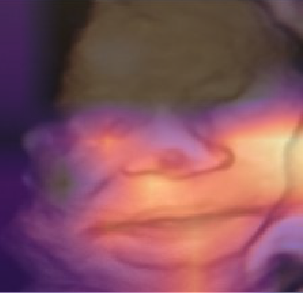
\includegraphics[width=0.32\textwidth]{imgs/chap6_gradcam.png}
    \caption{Grad-CAM heat map for visual explanations.}
    \label{fig:gradcam}
\end{figure}

It is important to highlight these explanations are an essential feature in an eventual application of our system in real life. As doctors and specialists look at the images produced by the model, the heat map should ideally agree with the indicators from pain scales and direct their view to regions of interest where manifestations of pain are present. We believe this feature would certainly give more robustness to the results and facilitate adoption by the users. As such, we stand out its importance and suggest further research as a future work topic in the next chapter.

\section{Answering Our Research Questions}

In this section, we aim to answer the proposed research questions from the beginning of this chapter based on the results we presented.

Regarding \textbf{RQ1}, we believe our results showed in tables \ref{tab:accuracy_all} and \ref{tab:accuracy_auc_ap} are a good argument to show it is viable to develop a learning model capable of effectively identifying pain. We believe an accuracy of 84.8\% is a good evidence that we are in the right direction, even considering that a new experiment with more data could be necessary to validate these conclusions any further. As data is complicated to collect, we think our experimental process was able to extract significant results out of it.

As for \textbf{RQ2}, we did see our model had problems in discriminating images of acute pain from those of an acoustic stimulus, although it did so very well from images of rest. It appears the images from acoustic stimulus indeed made the task more difficult, but we believe this effect would be mitigated if we had a larger dataset available for training. Nevertheless, even if we have a false positive predicted from an acoustic stimulus image, from a precautionary perspective, it would still benefit the fetus, as this could be an indication of discomfort and could also be treated.

Finally, for \textbf{RQ3}, it does appear transfer learning with pre-training in the VGGFace2 dataset performs better than when trained on ImageNet, as it achieved our best result. We believe this comes from the fact the pre-training on face images was able to learn features in their middle to last layers related to the human face, such as the mouth, the eyes, the chin, the nose. Even though the fetus images are relatively different, these features are still present, which could explain why the model detected them and performed better. 

